%how to: \input{res/chapters/argumentOfChapter}
%\section{Casi d'uso}
\begin{comment}
\subsection{Tipologia di utenti}
\subsection{Notazione Use Case}
\subsection{UC 1: Registrazione}
	\begin{figure}[htbp]
		\centering
		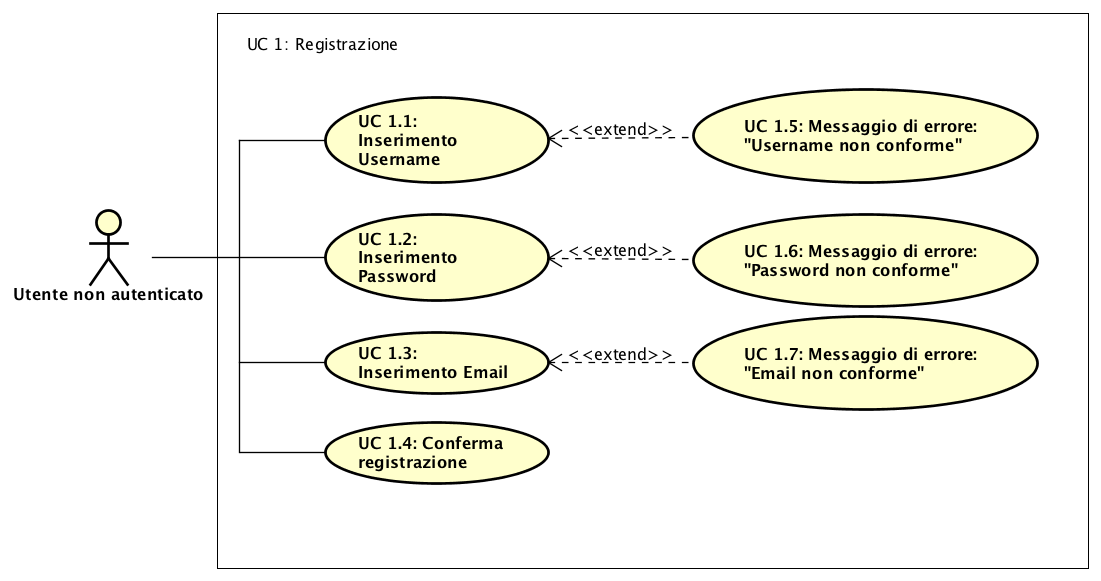
\includegraphics[scale=0.8]{../../Casi D'uso/UC1.png}
		\caption{Scelta della modalità di registrazione}
	\end{figure}
	\begin{itemize}
		\item \textbf{Attori coinvolti:} Utente non autenticato, che vuole interagire con il sistema. \\
		\item \textbf{Scopo e descrizione:} L'utente inserisce l'username che desidera utilizzare, la password che desidera utilizzare e uno dei propri indirizzi mail per effettuare la registrazione. \\
		\item \textbf{Precondizione:} Il sistema richiede all'utente le informazioni necessarie per effettuare la registrazione. \\
		\item \textbf{Postcondizione:} Il sistema elabora i dati inseriti dall'utente e, nel caso la registrazione avvenga con successo, gli concede la possibilità di accedere al sistema. In caso contrario viene visualizzato un messaggio d'errore e viene indicato dove è stato commesso, per l'appunto, l'errore. \\
	\end{itemize}
\subsection{UC 2: Autenticazione}
	\begin{figure}[h]
		\centering
		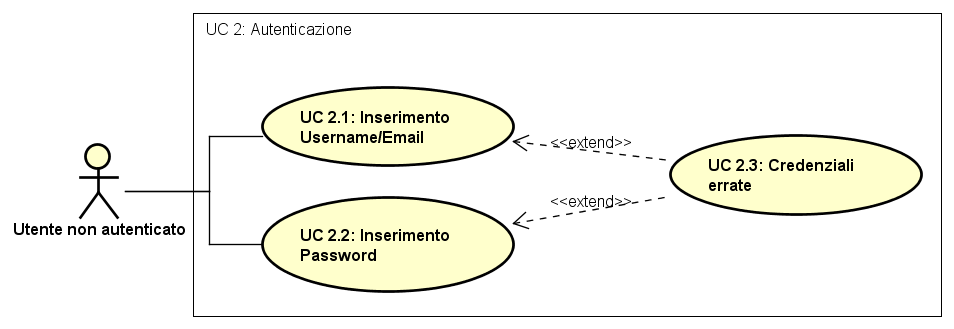
\includegraphics[scale=0.8]{../../Casi D'uso/UC2.png}
		\caption{Scelta della modalità di autenticazione}
	\end{figure}
	\begin{itemize}
		\item \textbf{Attori coinvolti:} Utente non autenticato, che vuole interagire con il sistema. \\
		\item \textbf{Scopo e descrizione:} L'utente inserisce il proprio username e la propria password per effettuare l'autenticazione. In caso di password dimenticata è possibile chiedere assistenza. \\
		\item \textbf{Precondizione:} L'utente decide di autenticarsi in maniera standard e il sistema richiede quindi l'inserimento delle informazioni necessarie per permettere l'operazione. \\
		\item \textbf{Postcondizione:} Il sistema elabora i dati forniti dall'utente e concede la possibilità di usufruire delle proprie funzionalità, se l'autenticazione avviene con successo. In caso contrario viene visualizzato un messaggio di autenticazione fallita e viene invitato l'utente a controllare i dati inseriti. \\
	\end{itemize}
\end{comment}
%\subsection{UC 4: Logout}
		
		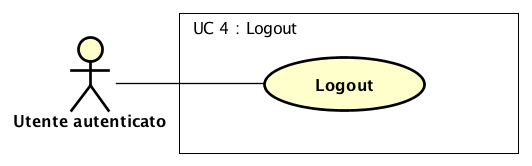
\includegraphics[scale=0.8]{../../Casi D'uso/UC4.png}
\begin{itemize}
		\item \textbf{Attori coinvolti:} Utente autenticato. \\
		\item \textbf{Scopo e descrizione:} L'utente autenticato pu\'o eseguire il logout dall’applicazione. \\
		\item \textbf{Precondizione:} L'applicazione offre all'utente la possibilit\'a di logout. \\
		\item \textbf{Postcondizione:}L'applicazione ha eseguito l'operazione di logout richiesta dall’utente. \\
\end{itemize}
%\subsection{UC 5: Gestione Progetti}
		\centering
		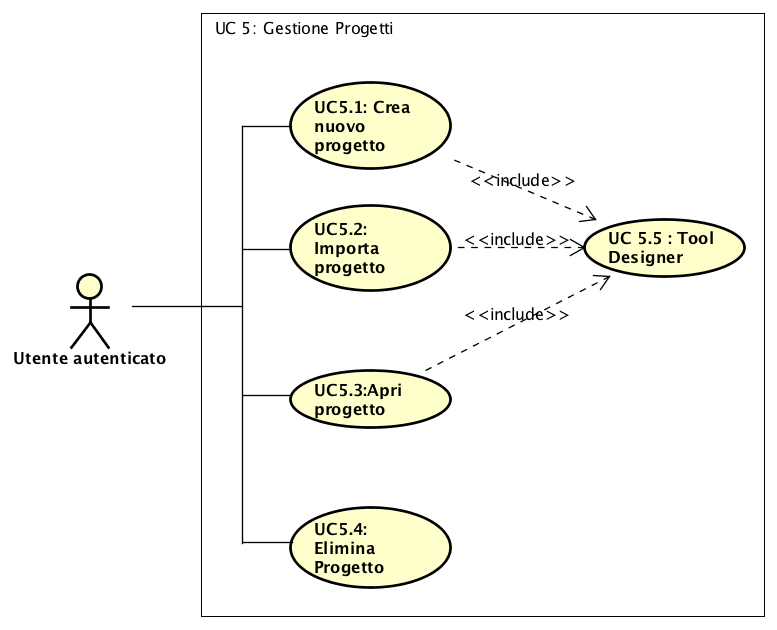
\includegraphics[scale=0.7]{../../Casi D'uso/UC5.png}
\begin{itemize}
		\item \textbf{Attori coinvolti:} Utente autenticato \\
		\item \textbf{Scopo e descrizione:} L'utente ha la possibilità di creare un nuovo progetto, modificare un progetto esistente, salvare un progetto o eliminare un progetto. \\
		\item \textbf{Precondizione:} L’applicazione visualizza i pulsanti predisposti per l’esecuzione di azioni sopra indicate. \\
		\item \textbf{Postcondizione:}L’applicazione, a seconda dell’azione scelta dall’utente, svolgerà le sue funzioni. \\
\end{itemize}

\section{Introduzione}
\subsection{Scopo del documento}
Lo scopo del documento è mostrare e descrivere le funzionalità che il prodotto dovrà avere. Tali requisiti sono emersi dal capitolato presentato, da discussioni interne, e da incontri svolti con il Proponente.

\subsection{Glossario}
          Con lo scopo di evitare ambiguità di linguaggio e di massimizzare la comprensione dei documenti, il
          gruppo ha steso un documento interno che è il \emph{Glossario v1.0.0}. In esso saranno definiti, in modo
          chiaro e conciso i termini che possono causare ambiguità o incomprensione del testo.
  \newpage        
\section{Riferimenti}
\subsection{Normativi}
\begin{itemize}
\item \textbf{Capitolato d'appalto C6:} SWEDesigner: editor di diagrammi \glossaryItem{UML} con generazione di codice \\
\url{http://www.math.unipd.it/~tullio/IS-1/2016/Progetto/C6p.pdf};
\item \textbf{Verbale di incontro} con il Proponente Zucchetti del 23-02-2017;
\item \textbf{Verbale di incontro} con il Proponente Zucchetti del 15-03-2017;
\item \textbf{Norme di Progetto v1.0.0}.
\end{itemize}
\subsection{Informativi}
\begin{itemize}
\item \textbf{Studio di Fattibilità v1.0.0};
\item \textbf{IEEE 830-1998}: \url{http://en.wikipedia.org/wiki/Software_requirements_specification}.
\item \textbf{Presentazione capitolato d'appalto}: \url{http://www.math.unipd.it/~tullio/IS-1/2016/Progetto/C6p.pdf}.
\end{itemize}
\newpage
\section{Descrizione generale}
\subsection{Contesto d'utilizzo}
Con il progetto SWEDesigner si vuole far avvicinare la fase di progettazione delle strutture delle classi, realizzata utilizzando i diagrammi delle classi previsti dell'UML, alla fase di creazione del corpo dei metodi, realizzata utilizzando i diagrammi delle attività previsti dall'UML, in modo da  rendere più forte la sincronizzazione tra questi due standard. In particolare il progetto intende creare un ambiente di sviluppo online per la creazione dei diagrammi sopra citati e la conseguente realizzazione del codice applicativo descritto dall'utente in fase di disegno.
 
\subsection{Funzione di Prodotto}
Le funzioni che saranno disponibili all'interno di SWEDesigner sono:
\begin{itemize}
\item Registrazione dell'utente per la visione dei propri progetti e dei template salvati; 
\item Creazione di un diagramma delle classi; 
\item Creazione di un diagramma delle attività per ogni metodo definito nelle classi;
\item Realizzazione del codice applicativo descritto tramite i diagrammi;
\item Gestione dei propri progetti;
\item Gestione dei propri template.
\end{itemize}

\subsection{Descrizione degli utenti}
Gli utenti che possono accedere al progetto SWEDesigner sono delle persone che hanno già esperienze nell'ambito della programmazione, in particolare conoscono le convenzioni dello standard UML riguardanti i diagrammi delle classi e delle attività. 
Per accedere alle funzionalità dell'applicazione l'utente dovrà effettuare una registrazione e successivamente un login, in modo da poter creare nuovi progetti e salvarli sul suo account.
\newpage
\section{Casi d'uso}
\subsubsection{UC1 - Registrazione} 
\label{sssec:UC1} 
\begin{itemize} 
\item \textbf{Attori}: Utente non autenticato.
\item \textbf{Descrizione}: L'attore desidera effettuare l'operazione di registrazione. Vengono richiesti dal sistema un username, univoco e conforme alle richieste, una password conforme alle richieste e una mail che rispetti il pattern predefinito.;
\item \textbf{Precondizione}: Il sistema richiede all'attore le informazioni necessarie per effettuare
la registrazione.;
\item \textbf{Postcondizione}: Il sistema ha elaborato i dati inseriti dall'attore e, nel caso la registrazione
sia avvenuta con successo, gli ha concesso la possibilità di accedere al sistema.
In caso contrario il sistema ha visualizzato un messaggio che illustra il tipo di errore che è stato commesso.;
\item \textbf{Scenario principale}: \begin{enumerate}\item Inserisci Username (UC1.1);\item Inserisci Password (UC1.2);\item Inserisci Email (UC1.3);\item Conferma registrazione (UC1.4);\item Messaggio errore: "Username non conforme" (UC1.5);\item Messaggio errore: "Password non conforme" (UC1.6);\item Messaggio errore: "Email non conforme" (UC1.7). 
 \end{enumerate}
\end{itemize} 
\subsubsection{UC1.1 - Inserisci Username} 
\label{sssec:UC1.1} 
\begin{itemize} 
\item \textbf{Attori}: Utente non autenticato.
\item \textbf{Descrizione}: L’attore inserisce l'username: deve essere univoco all'interno del sistema e deve essere alfanumerico.;
\item \textbf{Precondizione}: L'attore ha selezionato l'opzione di registrazione e non ha ancora inserito un username.;
\item \textbf{Postcondizione}: L'attore ha inserito un username conforme alle richieste del sistema.;
\end{itemize} 
\subsubsection{UC1.2 - Inserisci Password} 
\label{sssec:UC1.2} 
\begin{itemize} 
\item \textbf{Attori}: Utente non autenticato.
\item \textbf{Descrizione}: L’attore inserisce la password: deve essere di tipo alfanumerico e può contenere caratteri di punteggiatura.;
\item \textbf{Precondizione}: L'attore ha selezionato l'opzione di registrazione e non ha ancora inserito una password.;
\item \textbf{Postcondizione}: L'attore ha inserito una password conforme alle richieste del sistema.;
\end{itemize} 
\subsubsection{UC1.3 - Inserisci Email} 
\label{sssec:UC1.3} 
\begin{itemize} 
\item \textbf{Attori}: Utente non autenticato.
\item \textbf{Descrizione}: L’attore inserisce l'email, che deve essere scritta in maniera corretta.;
\item \textbf{Precondizione}: L'attore ha selezionato l'opzione di registrazione e non ha ancora inserito un email.;
\item \textbf{Postcondizione}: L'attore ha inserito un'email nel modo corretto.;
\end{itemize} 
\subsubsection{UC1.4 - Conferma registrazione} 
\label{sssec:UC1.4} 
\begin{itemize} 
\item \textbf{Attori}: Utente non autenticato.
\item \textbf{Descrizione}: Dopo che un attore ha effettuato correttamente una registrazione, gli viene inviato un messaggio di conferma.;
\item \textbf{Precondizione}: L'attore ha scelto di effettuare l'operazione di registrazione.;
\item \textbf{Postcondizione}: L'utente ha ricevuto un messaggio di conferma dell'avvenuta registrazione.;
\end{itemize} 
\subsubsection{UC1.5 - Messaggio errore: "Username non conforme"} 
\label{sssec:UC1.5} 
\begin{itemize} 
\item \textbf{Attori}: Utente non autenticato.
\item \textbf{Descrizione}: L'attore ha inserito un username non conforme e gli viene quindi comunicato l'errore.;
\item \textbf{Precondizione}: L'attore ha selezionato l'opzione di registrazione e ha inserito un username.;
\item \textbf{Postcondizione}: L'attore ha inserito un username non conforme e ha ricevuto la comunicazione dell'errore.;
\end{itemize} 
\subsubsection{UC1.6 - Messaggio errore: "Password non conforme"} 
\label{sssec:UC1.6} 
\begin{itemize} 
\item \textbf{Attori}: Utente non autenticato.
\item \textbf{Descrizione}: L'attore ha inserito una password non conforme e gli viene quindi comunicato l'errore.;
\item \textbf{Precondizione}: L'attore ha selezionato l'opzione di registrazione e ha inserito una password.;
\item \textbf{Postcondizione}: L'attore ha inserito una password non conforme e ha ricevuto la comunicazione dell'errore.;
\end{itemize} 
\subsubsection{UC1.7 - Messaggio errore: "Email non conforme"} 
\label{sssec:UC1.7} 
\begin{itemize} 
\item \textbf{Attori}: Utente non autenticato.
\item \textbf{Descrizione}: L'attore ha inserito un'email con una sintassi non valida e gli viene quindi comunicato l'errore.;
\item \textbf{Precondizione}: L'attore ha selezionato l'opzione di registrazione e ha inserito un'email.;
\item \textbf{Postcondizione}: L'attore ha inserito un'email non conforme e ha ricevuto la comunicazione dell'errore.;
\end{itemize} 
\subsubsection{UC2 - Autenticazione} 
\label{sssec:UC2} 
\begin{itemize} 
\item \textbf{Attori}: Utente non autenticato.
\item \textbf{Descrizione}: L'attore che già in possesso delle credenziali per accedere al sistema, potrà effettuare l'operazione di autenticazione inserendo l'username o l'email e la password utilizzati per l'autenticazione. Nel caso l’attore abbia perso la password o se la sia dimenticata, il sistema fornisce la possibilità di resettarla.;
\item \textbf{Precondizione}: L'attore decide di autenticarsi e il sistema richiede l'inserimento dei dati necessari per l'autenticazione.;
\item \textbf{Postcondizione}: L'attore ha avuto accesso alle funzionalità del sistema in caso l'autenticazione sia avvenuta con successo. In caso contrario il sistema ha visualizzato un messaggio d'errore.;
\item \textbf{Scenario principale}: \begin{enumerate}\item Inserisci Username/Email (UC2.1);\item Inserisci Password (UC2.2);\item Messaggio errore: "Username/Email o password errato" (UC2.4);\item Invio password per email (UC2.5). 
 \end{enumerate}
\end{itemize} 
\subsubsection{UC2.1 - Inserisci Username/Email} 
\label{sssec:UC2.1} 
\begin{itemize} 
\item \textbf{Attori}: Utente non autenticato.
\item \textbf{Descrizione}: Durante la fase di autenticazione viene richiesto all'attore il proprio username o la propria email.;
\item \textbf{Precondizione}: L'attore ha selezionato l'opzione di autenticazione e non ha ancora inserito il proprio username o la propria email.;
\item \textbf{Postcondizione}: L'attore ha inserito il proprio username o la propria email.;
\end{itemize} 
\subsubsection{UC2.2 - Inserisci Password} 
\label{sssec:UC2.2} 
\begin{itemize} 
\item \textbf{Attori}: Utente non autenticato.
\item \textbf{Descrizione}: Durante la fase di autenticazione viene richiesta all'attore la propria password.;
\item \textbf{Precondizione}: L'utente ha selezionato l'opzione di autenticazione e non ha ancora inserito la propria password.;
\item \textbf{Postcondizione}: L'attore ha inserito la propria email.;
\end{itemize} 
\subsubsection{UC2.4 - Messaggio errore: "Username/Email o password errato"} 
\label{sssec:UC2.4} 
\begin{itemize} 
\item \textbf{Attori}: Utente non autenticato.
\item \textbf{Descrizione}: L'attore, già in possesso delle credenziali d'accesso, tenta di autenticarsi, ma l'operazione non va a buon fine e viene visualizzato un messaggio d'errore.;
\item \textbf{Precondizione}: L'attore ha intenzione di effettuare l'operazione di autenticazione ed ha inserito il proprio username o la propria email.;
\item \textbf{Postcondizione}: Il sistema ha ricevuto informazioni errate e quindi ha mostrato un messaggio d'errore.;
\end{itemize} 
\subsubsection{UC2.5 - Invio password per email} 
\label{sssec:UC2.5} 
\begin{itemize} 
\item \textbf{Attori}: Utente non autenticato.
\item \textbf{Descrizione}: Se l'attore ha perso oppure ha dimenticato la propria password, il sistema fornisce uno strumento per riceverne una nuova.;
\item \textbf{Precondizione}: L'attore è in possesso di un account all'interno del sistema, ma non ricorda più la password.;
\item \textbf{Postcondizione}: L'attore ha ricevuto una nuova email contenente una nuova password temporanea.;
\end{itemize} 
\subsubsection{UC3 - Gestione Profilo} 
\label{sssec:UC3} 
\begin{itemize} 
\item \textbf{Attori}: Utente Autenticato.
\item \textbf{Descrizione}: L' attore vuole gestire il suo username, la sua password o il suo indirizzo e-mail.;
\item \textbf{Precondizione}: L' attore ha già effettuato l'accesso e l'applicazione rende disponibile la voce Gestione Profilo.;
\item \textbf{Postcondizione}: L' applicazione visualizza i dati dell'attore con gli opportuni pulsanti di modifica.;
\item \textbf{Scenario principale}: \begin{enumerate}\item Modifica Username (UC3.1);\item Modifica Password (UC3.2);\item Modifica Email (UC3.3). 
 \end{enumerate}
\end{itemize} 
\subsubsection{UC3.1 - Modifica Username} 
\label{sssec:UC3.1} 
\begin{itemize} 
\item \textbf{Attori}: Utente Autenticato.
\item \textbf{Descrizione}: L' attore può modificare il suo nome utente.;
\item \textbf{Precondizione}: L' applicazione deve rendere disponibile il pulsante di modifica username.;
\item \textbf{Postcondizione}: L' applicazione modifica l'username dell'attore.;
\end{itemize} 
\subsubsection{UC3.2 - Modifica Password} 
\label{sssec:UC3.2} 
\begin{itemize} 
\item \textbf{Attori}: Utente Autenticato.
\item \textbf{Descrizione}: L' attore ha la possibilità di modificare la sua password.;
\item \textbf{Precondizione}: L' applicazione rende disponibile il pulsante di modifica.;
\item \textbf{Postcondizione}: L' applicazione modifica la password o restituisce il messaggio d'errore.;
\end{itemize} 
\subsubsection{UC3.3 - Modifica Email} 
\label{sssec:UC3.3} 
\begin{itemize} 
\item \textbf{Attori}: Utente Autenticato.
\item \textbf{Descrizione}: L' attore ha la possibilità di modificare la propria email.;
\item \textbf{Precondizione}: L' applicazione rende disponibile il pulsante per la modifica della email.;
\item \textbf{Postcondizione}: L' applicazione aggiorna la nuova email.;
\end{itemize} 
\subsubsection{UC4 - Logout} 
\label{sssec:UC4} 
\begin{itemize} 
\item \textbf{Attori}: Utente Autenticato.
\item \textbf{Descrizione}: L' attore può effettuare il logout dal suo profilo.;
\item \textbf{Precondizione}: L' applicazione offre il pulsante di logout visibile all'utente che ha effettuato l'accesso.;
\item \textbf{Postcondizione}: L' applicazione effettua il logout dell'attore.;
\end{itemize} 
\subsubsection{UC5 - Gestione Progetti} 
\label{sssec:UC5} 
\begin{itemize} 
\item \textbf{Attori}: Utente Autenticato.
\item \textbf{Descrizione}: L’ attore ha la possibilità di aggiungere un nuovo progetto e di aprire o modificare un progetto già esistente.;
\item \textbf{Precondizione}: L’ applicazione visualizza i pulsanti predisposti per l’esecuzione delle azioni sopra indicate.;
\item \textbf{Postcondizione}: L’ applicazione, a seconda dell’azione scelta dall’utente, svolgerà le sue funzioni;
\item \textbf{Scenario principale}: \begin{enumerate}\item Aggiunta Progetto (UC5.1);\item Apri progetto (UC5.2);\item Elimina Progetto (UC5.3). 
 \end{enumerate}
\end{itemize} 
\subsubsection{UC5.1 - Aggiunta Progetto} 
\label{sssec:UC5.1} 
\begin{itemize} 
\item \textbf{Attori}: Utente Autenticato.
\item \textbf{Descrizione}: L’ attore ha la possibilità di creare un nuovo progetto.;
\item \textbf{Precondizione}: L’applicazione rende disponibile il pulsante aggiungi progetti.;
\item \textbf{Postcondizione}: L’applicazione apre un nuovo foglio per la realizzazione del nuovo progetto.;
\end{itemize} 
\subsubsection{UC5.2 - Apri progetto} 
\label{sssec:UC5.2} 
\begin{itemize} 
\item \textbf{Attori}: Utente Autenticato.
\item \textbf{Descrizione}: L’ attore ha la possibilità di aprire un progetto precedentemente salvato.;
\item \textbf{Precondizione}: L’ applicazione rende disponibile il pulsante apri progetto, se precedentemente ne era stato salvato almeno uno.;
\item \textbf{Postcondizione}: L’applicazione apre il progetto selezionato.;
\end{itemize} 
\subsubsection{UC5.3 - Elimina Progetto} 
\label{sssec:UC5.3} 
\begin{itemize} 
\item \textbf{Attori}: Utente Autenticato.
\item \textbf{Descrizione}: L' attore ha la possibilità di eliminare un progetto precedentemente salvato.;
\item \textbf{Precondizione}: L’applicazione rende disponibile il pulsante elimina progetto, se precedentemente ne era stato salvato almeno uno.;
\item \textbf{Postcondizione}: L’applicazione elimina il progetto selezionato.;
\end{itemize} 
\subsubsection{UC6 - Tool Designer} 
\label{sssec:UC6} 
\begin{itemize} 
\item \textbf{Attori}: .
\item \textbf{Descrizione}: Tool Designer;
\item \textbf{Precondizione}: Tool Designer;
\item \textbf{Postcondizione}: Tool Designer;
\item \textbf{Scenario principale}: \begin{enumerate}\item Menù (UC6.1);\item Toolbar (UC6.2);\item Disegnatore diagrammi (UC6.3);\item Pannello laterale (UC6.4). 
 \end{enumerate}
\end{itemize} 
\subsubsection{UC6.1 - Menù} 
\label{sssec:UC6.1} 
\begin{itemize} 
\item \textbf{Attori}: Utente Autenticato.
\item \textbf{Descrizione}: L’ attore può accedere alle voci file, edit, tool,
layers e window appartenenti al menù del tool designer.;
\item \textbf{Precondizione}: L’applicazione offre all’utente una barra dei menù.;
\item \textbf{Postcondizione}: L’applicazione, a seconda dell’operazione richiesta dall’utente,
svolge le sue funzioni.;
\item \textbf{Scenario principale}: \begin{enumerate}\item File (UC6.1.1);\item Edit (UC6.1.2);\item Template (UC6.1.3);\item Layers (UC6.1.4). 
 \end{enumerate}
\end{itemize} 
\subsubsection{UC6.1.1 - File} 
\label{sssec:UC6.1.1} 
\begin{itemize} 
\item \textbf{Attori}: Utente Autenticato.
\item \textbf{Descrizione}: L’attore può accedere alle voci salva, chiudi, esporta, genera codice e salva template appartenenti alla voce file del menù.;
\item \textbf{Precondizione}: L’applicazione offre all’utente la voce file nella barra dei menù.;
\item \textbf{Postcondizione}: L’applicazione, a seconda dell’operazione richiesta dall’utente,
svolge le sue funzioni.;
\item \textbf{Scenario principale}: \begin{enumerate}\item Salva (UC6.1.1.1);\item Chiudi (UC6.1.1.2);\item Esporta (UC6.1.1.3);\item Genera codice (UC6.1.1.4);\item Salva template (UC6.1.1.5). 
 \end{enumerate}
\end{itemize} 
\subsubsection{UC6.1.1.1 - Salva} 
\label{sssec:UC6.1.1.1} 
\begin{itemize} 
\item \textbf{Attori}: Utente Autenticato.
\item \textbf{Descrizione}: L’attore può salvare il suo progetto nello stato
corrente.;
\item \textbf{Precondizione}: L’applicazione offre all’utente il salvataggio, disponibile alla voce salva del file appartenente alla barra del menù.;
\item \textbf{Postcondizione}: L’applicazione salva il progetto nello stato corrente.;
\end{itemize} 
\subsubsection{UC6.1.1.2 - Chiudi} 
\label{sssec:UC6.1.1.2} 
\begin{itemize} 
\item \textbf{Attori}: Utente Autenticato.
\item \textbf{Descrizione}: L’attore può chiudere il progetto corrente.;
\item \textbf{Precondizione}: L’applicazione offre all’attore la chiusura del progetto, disponibile
alla voce chiudi del menù.;
\item \textbf{Postcondizione}: L’applicazione chiude il progetto corrente.;
\end{itemize} 
\subsubsection{UC6.1.1.3 - Esporta} 
\label{sssec:UC6.1.1.3} 
\begin{itemize} 
\item \textbf{Attori}: Utente Autenticato.
\item \textbf{Descrizione}: L’attore può esportare il progetto corrente in
un altro formato.;
\item \textbf{Precondizione}: L’applicazione offre all’attore la possibilità di esportare il progetto,
selezionando la voce esporta nel menù.;
\item \textbf{Postcondizione}: L’applicazione esporta il progetto.;
\end{itemize} 
\subsubsection{UC6.1.1.4 - Genera codice} 
\label{sssec:UC6.1.1.4} 
\begin{itemize} 
\item \textbf{Attori}: Utente Autenticato.
\item \textbf{Descrizione}: L’attore può generare il codice relativo all’UML
prodotto.;
\item \textbf{Precondizione}: L’applicazione offre all’utente la possibilità di generare il codice
relativo all’UML, alla voce genera codice del menù.;
\item \textbf{Postcondizione}: L’applicazione genera il codice relativo al disegno UML.;
\end{itemize} 
\subsubsection{UC6.1.1.5 - Salva template} 
\label{sssec:UC6.1.1.5} 
\begin{itemize} 
\item \textbf{Attori}: Utente Autenticato.
\item \textbf{Descrizione}: L’attore ha la possibilità di salvare determinate classi o gerarchie, aggiungendole così alla lista di template già salvati.;
\item \textbf{Precondizione}: L’applicazione offre all’utente la voce salva template, sottovoce di file nel menù, solamente se sono state create una o più classi, ed ognuna di esse ha un commento che le identifica.;
\item \textbf{Postcondizione}: Viene aggiunto alla lista dei template il template desiderato.;
\end{itemize} 
\subsubsection{UC6.1.2 - Edit} 
\label{sssec:UC6.1.2} 
\begin{itemize} 
\item \textbf{Attori}: Utente Autenticato.
\item \textbf{Descrizione}: L’attore può accedere alle voci annulla, ripristina, taglia, copia, incolla, zoom in e zoom out appartenenti alla voce edit del menù.;
\item \textbf{Precondizione}: L’applicazione offre all’utente la voce edit appartenente barra
dei menù.;
\item \textbf{Postcondizione}: L’applicazione, a seconda dell’operazione richiesta dall’utente,
effettua la modifica.;
\item \textbf{Scenario principale}: \begin{enumerate}\item Annulla (UC6.1.2.1);\item Ripristina (UC6.1.2.2);\item Taglia (UC6.1.2.3);\item Copia (UC6.1.2.4);\item Incolla (UC6.1.2.5);\item Zoom in (UC6.1.2.6);\item Zoom out (UC6.1.2.7). 
 \end{enumerate}
\end{itemize} 
\subsubsection{UC6.1.2.1 - Annulla} 
\label{sssec:UC6.1.2.1} 
\begin{itemize} 
\item \textbf{Attori}: Utente Autenticato.
\item \textbf{Descrizione}: L’attore può tornare allo stato precedente l’ultima
modifica.;
\item \textbf{Precondizione}: L’applicazione offre all’utente la possibilità di selezionare la voce
annulla, sottovoce di edit nella barra del menù.;
\item \textbf{Postcondizione}: L’applicazione torna allo stato precedente l’ultima modifica.;
\end{itemize} 
\subsubsection{UC6.1.2.2 - Ripristina} 
\label{sssec:UC6.1.2.2} 
\begin{itemize} 
\item \textbf{Attori}: Utente Autenticato.
\item \textbf{Descrizione}: L’attore può ripristinare le modifiche effettuate
successivamente allo stato attuale.;
\item \textbf{Precondizione}: L’applicazione offre all’utente la possibilità di selezionare la voce
ripristina, sottovoce di edit nella barra del menù, solamente se si era tornati ad uno
stato precedente all’ultima modifica.;
\item \textbf{Postcondizione}: L’applicazione torna allo stato precedente l’ultima modifica.;
\end{itemize} 
\subsubsection{UC6.1.2.3 - Taglia} 
\label{sssec:UC6.1.2.3} 
\begin{itemize} 
\item \textbf{Attori}: Utente Autenticato.
\item \textbf{Descrizione}: L’attore può tagliare un determinato elemento
del progetto.;
\item \textbf{Precondizione}: L’applicazione offre all’utente la voce taglia, sottovoce di edit appartenente
al menù.;
\item \textbf{Postcondizione}: L’applicazione taglia l’elemento selezionato.;
\end{itemize} 
\subsubsection{UC6.1.2.4 - Copia} 
\label{sssec:UC6.1.2.4} 
\begin{itemize} 
\item \textbf{Attori}: Utente Autenticato.
\item \textbf{Descrizione}: L’attore può copiare un determinato elemento
del progetto.;
\item \textbf{Precondizione}: L’applicazione offre all’utente la voce copia, sottovoce di edit appartenente
al menù.;
\item \textbf{Postcondizione}: L’applicazione copia l’elemento selezionato.;
\end{itemize} 
\subsubsection{UC6.1.2.5 - Incolla} 
\label{sssec:UC6.1.2.5} 
\begin{itemize} 
\item \textbf{Attori}: Utente Autenticato.
\item \textbf{Descrizione}: L’attore può incollare un elemento precedentemente
tagliato o copiato.;
\item \textbf{Precondizione}: L’applicazione offre all’utente la possibilità di selezionare la voce
incolla, sottovoce di edit appartenente a menù, se un elemento era stato copiato o
tagliato precedentemente .;
\item \textbf{Postcondizione}: L’applicazione inserisce l’elemento designato.;
\end{itemize} 
\subsubsection{UC6.1.2.6 - Zoom in} 
\label{sssec:UC6.1.2.6} 
\begin{itemize} 
\item \textbf{Attori}: Utente Autenticato.
\item \textbf{Descrizione}: L’attore può ingrandire la visualizzazione di
una determinata sezione.;
\item \textbf{Precondizione}: L’applicazione offre all’utente la possibilità di selezionare la voce
zoom in, sottovoce di edit appartenente al menù.;
\item \textbf{Postcondizione}: L’applicazione ingrandisce la sezione prescelta.;
\end{itemize} 
\subsubsection{UC6.1.2.7 - Zoom out} 
\label{sssec:UC6.1.2.7} 
\begin{itemize} 
\item \textbf{Attori}: Utente Autenticato.
\item \textbf{Descrizione}: L’attore può rimpicciolire la visualizzazione di
una determinata sezione.;
\item \textbf{Precondizione}: L’applicazione offre all’utente la possibilità di selezionare la voce
zoom out, sottovoce di edit appartenente al menù.;
\item \textbf{Postcondizione}: L’applicazione rimpicciolisce la sezione prescelta.;
\end{itemize} 
\subsubsection{UC6.1.3 - Template} 
\label{sssec:UC6.1.3} 
\begin{itemize} 
\item \textbf{Attori}: .
\item \textbf{Descrizione}: L’utente autenticato può accedere alla visualizzazione della lista dei template. I template visualizzati comprendono sia quelli già dati dagli sviluppatore, sia i propri template.;
\item \textbf{Precondizione}: L’applicazione offre all’utente una barra dei menù.;
\item \textbf{Postcondizione}: L'applicazione ha aperto una finestra dove viene visualizzata la lista dei template e fornisce la possibilità di inserimento od eliminazione.;
\item \textbf{Scenario principale}: \begin{enumerate}\item Inserisci template (UC6.1.3.1);\item Elimina template (UC6.1.3.2). 
 \end{enumerate}
\end{itemize} 
\subsubsection{UC6.1.3.1 - Inserisci template} 
\label{sssec:UC6.1.3.1} 
\begin{itemize} 
\item \textbf{Attori}: .
\item \textbf{Descrizione}: L'utente inserisce nella finestra del disegnatore dei diagrammi ( UC 6.3 ) il template selezionato.;
\item \textbf{Precondizione}: L'utente ha aperto la finestra di gestione dei template.;
\item \textbf{Postcondizione}: L'utente aggiunge il template selezionato nella finestra del disegnatore dei diagrammi( UC 6.3 ).;
\item \textbf{Scenario principale}: L'utente seleziona il template desiderato da inserire.
L'utente clicca nella finestra del disegnatore dei diagrammi( UC 6.3 ) nel punto dove inserire il template.;\item \textbf{Scenari alternativi}: L'utente chiude la finestra di gestione template ( UC 6.1.3 ) e non viene effettuata nessuna operazione..
\end{itemize} 
\subsubsection{UC6.1.3.2 - Elimina template} 
\label{sssec:UC6.1.3.2} 
\begin{itemize} 
\item \textbf{Attori}: .
\item \textbf{Descrizione}: L'utente elimina dalla lista il template selezionato.;
\item \textbf{Precondizione}: L'utente ha aperto la finestra di gestione dei template ( UC 6.1.3 ).;
\item \textbf{Postcondizione}: Il template selezionato viene rimosso dalla lista.;
\item \textbf{Scenario principale}: L'utente seleziona il template desiderato da eliminare.
L'utente clicca il bottone nella stessa linea rappresentato da una "X".
Viene fatta una richiesta di conferma di eliminazione.
Tale template viene eliminato dalla lista se la conferma ha esito positivo.;\item \textbf{Scenari alternativi}: L'utente chiude la finestra di gestione template ( UC 6.1.3 ) e non viene effettuata nessuna operazione..
\end{itemize} 
\subsubsection{UC6.1.4 - Layers} 
\label{sssec:UC6.1.4} 
\begin{itemize} 
\item \textbf{Attori}: Utente Autenticato.
\item \textbf{Descrizione}: L’utente autenticato può accedere alla visualizzazione della lista dei layers. Può inoltre creare nuovi layer oppure rinominarne o eliminarne di già esistenti.;
\item \textbf{Precondizione}: L’applicazione offre all’utente una barra dei menù.;
\item \textbf{Postcondizione}: L'applicazione ha eseguito l'operazione richiesta dallutente.;
\item \textbf{Scenario principale}: \begin{enumerate}\item Nuovo (UC6.1.4.1);\item Lista (UC6.1.4.2);\item Modifica (UC6.1.4.3). 
 \end{enumerate}
\end{itemize} 
\subsubsection{UC6.1.4.1 - Nuovo} 
\label{sssec:UC6.1.4.1} 
\begin{itemize} 
\item \textbf{Attori}: Utente Autenticato.
\item \textbf{Descrizione}: L'utente crea un nuovo layer a cui è possibile assegnare delle classi.;
\item \textbf{Precondizione}: L'utente ha aperto la finestra di gestione dei layer.;
\item \textbf{Postcondizione}: L'utente ha aggiunto un nuovo layer assegnandogli il nome desiderato.;
\end{itemize} 
\subsubsection{UC6.1.4.2 - Lista} 
\label{sssec:UC6.1.4.2} 
\begin{itemize} 
\item \textbf{Attori}: Utente Autenticato.
\item \textbf{Descrizione}: L'utente seleziona il layer di cui desidera visualizzare le classi che gli sono state assegnate.;
\item \textbf{Precondizione}: L'utente ha aperto la finestra di gestione dei layer.;
\item \textbf{Postcondizione}: L'utente ha visualizzato le classi assegnate al layer desiderato.;
\end{itemize} 
\subsubsection{UC6.1.4.3 - Modifica} 
\label{sssec:UC6.1.4.3} 
\begin{itemize} 
\item \textbf{Attori}: Utente Autenticato.
\item \textbf{Descrizione}: L'utente desidera rinominare oppure eliminare un layer tra quelli esistenti.;
\item \textbf{Precondizione}: L'utente ha aperto la finestra di gestione dei layer.;
\item \textbf{Postcondizione}: L'utente ha eseguito l'operazione desiderata.;
\item \textbf{Scenario principale}: \begin{enumerate}\item Rinomina (UC6.1.4.3.1);\item Elimina (UC6.1.4.3.2). 
 \end{enumerate}
\end{itemize} 
\subsubsection{UC6.1.4.3.1 - Rinomina} 
\label{sssec:UC6.1.4.3.1} 
\begin{itemize} 
\item \textbf{Attori}: Utente Autenticato.
\item \textbf{Descrizione}: L'utente desidera rinominare un layer tra quelli esistenti.;
\item \textbf{Precondizione}: L'utente ha aperto la finestra di gestione dei layer e ha selezionato l'opzione di modifica.;
\item \textbf{Postcondizione}: L'utente ha modificato il nome del layer che intendeva modificare, mantenendo tutte le classi associate.;

\newpage
\section{Requisiti}
\subsection{Requisiti funzionali}
\def\arraystretch{1.5}
\rowcolors{2}{D}{P}
\begin{longtable}{p{2cm}!{\VRule[1pt]}p{2cm}!{\VRule[1pt]}p{5cm}!{\VRule[1pt]}p{1.5cm}}
\rowcolor{I}
\color{white} \textbf{Requisito} & \color{white} \textbf{Tipologia} & \color{white} \textbf{Descrizione} & \color{white} \textbf{Fonti} \\ 
\endfirsthead 
\rowcolor{I} 
\color{white} \textbf{Requisito} & \color{white} \textbf{Tipologia} & \color{white} \textbf{Descrizione} & \color{white} \textbf{Fonti} \\ 
\endhead 
R0F1&Funzionale\newline Obbligatorio & L'attore deve registrarsi per accedere ai servizi forniti dal  programma & Interno \newline UC1
 \\
R0F1.1&Funzionale\newline Obbligatorio & L'attore deve inserire un username univoco & Interno \newline UC1
 \newline UC1.1
 \\
R0F1.2&Funzionale\newline Obbligatorio & L'attore deve inserire una password & Interno \newline UC1.2
 \\
R0F1.3&Funzionale\newline Obbligatorio & L'attore deve inserire una email & Interno \newline UC1
 \newline UC1.3
 \\
R0F1.4&Funzionale\newline Obbligatorio & L'attore può confermare la registrazione & Interno \newline UC1
 \newline UC1.4
 \\
R0F1.5&Funzionale\newline Obbligatorio & L'applicazione deve visualizzare un messaggio d'errore se l'username non è conforme alle richieste & Interno \newline UC1
 \newline UC1.5
 \\
R0F1.6&Funzionale\newline Obbligatorio & L'applicazione deve visualizzare un messaggio d'errore se la password non è conforme alle richieste & Interno \newline UC1
 \newline UC1.6
 \\
R0F1.7&Funzionale\newline Obbligatorio & L'applicazione deve visualizzare un messaggio d'errore se l'email non è conforme alle richieste & Interno \newline UC1
 \newline UC1.7
 \\
R0F2&Funzionale\newline Obbligatorio & L'attore per accedere ai servizi forniti deve aver effettuato l'autenticazione e diventare utente autenticato & Interno \newline UC2
 \\
R0F2.1&Funzionale\newline Obbligatorio & L'attore deve inserire il proprio Username o Email utilizzati in fase di registrazione & Interno \newline UC2
 \newline UC2.1
 \\
R0F2.2&Funzionale\newline Obbligatorio & L'attore deve inserire il propria password utilizzata in fase di registrazione & Interno \newline UC2
 \newline UC2.2
 \\
R0F2.4&Funzionale\newline Obbligatorio & L'applicazione visualizza un messaggio di errore dato dall'inserimento di credenziali errate & Interno \newline UC2
 \newline UC2.4
 \\
R1F2.3&Funzionale\newline Desiderabile & L'attore può accedere alla pagina per il recupero della password & Interno \newline UC2
 \newline UC2.3
 \\
R1F2.5&Funzionale\newline Desiderabile & L'applicazione invia la password all'indirizzo email inserito durante registrazione & Interno \newline UC2
 \newline UC2.5
 \\
R0F4&Funzionale\newline Obbligatorio & L'attore esce dal suo profilo & Interno \newline UC4
 \\
R0F5&Funzionale\newline Obbligatorio & L'attore visualizza l'elenco dei suoi progetti & Interno \newline UC5
 \\
R0F5.1&Funzionale\newline Obbligatorio & L'attore aggiunge un nuovo progetto & Interno \newline UC5
 \newline UC5.1
 \\
R0F5.1.1&Funzionale\newline Obbligatorio & L'attore crea un nuovo progetto vuoto & Interno \newline UC5.1
 \newline UC5.1.1
 \\
R0F5.1.2&Funzionale\newline Obbligatorio & L'attore importa un progetto & Interno \newline UC5.1
 \newline UC5.1.2
 \\
R0F5.2&Funzionale\newline Obbligatorio & L'attore  apre un progetto precedentemente salvato & Interno \newline UC5
 \newline UC5.2
 \\
R0F5.3&Funzionale\newline Obbligatorio & L'attore elimina un progetto precedentemente salvato & Interno \newline UC5
 \newline UC5.3
 \\
R0F6&Funzionale\newline Obbligatorio & L'applicazione visualizza l'editor dei diagrammi & Interno \newline UC6
 \\
R0F6.1&Funzionale\newline Obbligatorio & L'applicazione visualizza la barra del menu & Interno \newline UC6
 \newline UC6.1
 \\
R0F6.1.1&Funzionale\newline Obbligatorio & L'applicazione visualizza le voci presenti nel menu File & Interno \newline UC6.1
 \newline UC6.1.1
 \\
R0F6.1.1.1&Funzionale\newline Obbligatorio & L'attore può salvare il progetto in uso & Interno \newline UC6.1.1
 \newline UC6.1.1.1
 \\
R0F6.1.1.2&Funzionale\newline Obbligatorio & L'attore può chiudere il progetto in uso & Interno \newline UC6.1
 \newline UC6.1.1.2
 \\
R0F6.1.1.3&Funzionale\newline Obbligatorio & L'attore può esportare il progetto in uso & Interno \newline UC6.1
 \newline UC6.1.1.3
 \\
R0F6.1.1.4&Funzionale\newline Obbligatorio & L'attore può selezionare la generazione del codice  & Capitolato \newline UC6.1.1
 \newline UC6.1.1.4
 \\
R1F6.1.1.5&Funzionale\newline Desiderabile & L'attore può salvare il progetto corrente come template & Riunione esterna \\
R1F6.1.2&Funzionale\newline Desiderabile & L'applicazione visualizza le voci presenti nel menu Edit & Interno \newline UC6.1
 \newline UC6.1.2
 \\
R1F6.1.2.1&Funzionale\newline Desiderabile & L'attore può annullare l'ultima operazione effettuata & Interno \newline UC6.1.2
 \newline UC6.1.2.1
 \\
R1F6.1.2.2&Funzionale\newline Desiderabile & L'attore può ripristinare l'ultima operazione effettuata & Interno \newline UC6.1.2
 \newline UC6.1.2.2
 \\
R1F6.1.2.3&Funzionale\newline Desiderabile & L'attore può effettuare l'operazione "taglia" di un oggetto selezionato & Interno \newline UC6.1.2
 \newline UC6.1.2.3
 \\
R1F6.1.2.4&Funzionale\newline Desiderabile & L'attore può effettuare l'operazione "copia" di un oggetto selezionato & Interno \newline UC6.1.2
 \newline UC6.1.2.4
 \\
R1F6.1.2.5&Funzionale\newline Desiderabile & L'attore può effettuare l'operazione "incolla" di un oggetto precedentemente copiato & Interno \newline UC6.1.2
 \newline UC6.1.2.5
 \\
R1F6.1.2.6&Funzionale\newline Desiderabile & L'attore può effettuare l'operazione "zoom-in" della schermata & Interno \newline UC6.1.2
 \newline UC6.1.2.6
 \\
R1F6.1.2.7&Funzionale\newline Desiderabile & L'attore può effettuare l'operazione "zoom-out" della schermata & Interno \newline UC6.1.2
 \newline UC6.1.2.7
 \\
R1F6.1.3&Funzionale\newline Desiderabile & L'applicazione visualizza l'elenco dei template disponibili & Interno \newline UC6.1
 \newline UC6.1.3
 \\
R1F6.1.3.1&Funzionale\newline Desiderabile & L'attore può aggiungere al proprio progetto un template & Riunione esterna \newline UC6.1.3
 \newline UC6.1.3.1
 \\
R1F6.1.3.2&Funzionale\newline Desiderabile & L'attore può eliminare un proprio template precedentemente salvato & Interno \newline UC6.1.3
 \newline UC6.1.3.2
 \\
R2F6.1.4&Funzionale\newline Opzionale & L'applicazione visualizza le voci presenti nel menu Layers & Riunione esterna \newline UC6.1
 \newline UC6.1.4
 \\
R2F6.1.4.1&Funzionale\newline Opzionale & L'attore può creare un nuovo layer & Interno \newline UC6.1.4
 \newline UC6.1.4.1
 \\
R2F6.1.4.2&Funzionale\newline Opzionale & L'attore seleziona i layers che vuole visionare nella lista visualizzata dal sistema & Interno \newline UC6.1.4
 \newline UC6.1.4.2
 \\
R2F6.1.4.3&Funzionale\newline Opzionale & L'attore può modificare i layers presenti & Interno \newline UC6.1.4
 \newline UC6.1.4.3
 \\
R2F6.1.4.3.1&Funzionale\newline Opzionale & L'attore può modificare il nome del layer & Interno \newline UC6.1.4.3
 \newline UC6.1.4.3.1
 \\
R2F6.1.4.3.2&Funzionale\newline Opzionale & L'attore può eliminare un layer & Interno \newline UC6.1.4.3
 \newline UC6.1.4.3.2
 \\
R0F6.2&Funzionale\newline Obbligatorio & L'applicazione visualizza la barra degli strumenti grafici & Interno \newline UC6
 \newline UC6.2
 \\
R0F6.2.1&Funzionale\newline Obbligatorio & L'applicazione visualizza il menu per il disegno dei diagrammi delle classi & Capitolato \newline UC6.2
 \newline UC6.2.1
 \\
R0F6.2.1.1&Funzionale\newline Obbligatorio & L'attore può aggiungere un nuovo elemento di tipo "classe" & Interno \newline UC6.2.1
 \newline UC6.2.1.1
 \\
R0F6.2.1.2&Funzionale\newline Obbligatorio & L'attore può aggiungere un nuovo elemento di tipo "pacchetto" & Interno \newline UC6.2.1
 \newline UC6.2.1.2
 \\
R0F6.2.1.3&Funzionale\newline Obbligatorio & L'attore può aggiungere un nuovo elemento di tipo "relazione" & Interno \newline UC6.2.1
 \newline UC6.2.1.3
 \\
R0F6.2.1.3.1&Funzionale\newline Obbligatorio & L'attore seleziona la classe di partenza della relazione & Interno \newline UC6.2.1.3
 \newline UC6.2.1.3.1
 \\
R0F6.2.1.3.2&Funzionale\newline Obbligatorio & L'attore seleziona la classe di destinazione della relazione & Interno \newline UC6.2.1.3
 \newline UC6.2.1.3.2
 \\
R0F6.2.1.3.3&Funzionale\newline Obbligatorio & L'attore seleziona il tipo di relazione da inserire & Interno \newline UC6.2.1.3
 \newline UC6.2.1.3.3
 \\
R0F6.2.1.4&Funzionale\newline Obbligatorio & L'attore può aggiungere un nuovo elemento di tipo "commento" & Interno \newline UC6.2.1
 \newline UC6.2.1.4
 \\
R0F6.2.1.4.1&Funzionale\newline Obbligatorio & L'attore seleziona la classe a cui è associato il commento & Interno \newline UC6.2.1.4
 \newline UC6.2.1.4.1
 \\
R0F6.2.2&Funzionale\newline Obbligatorio & L'applicazione visualizza il menu per il disegno dei diagrammi delle attività & Capitolato \newline UC6.2
 \newline UC6.2.2
 \\
R0F6.2.2.1&Funzionale\newline Obbligatorio & L'attore può aggiungere un nuovo elemento di tipo "operazione" & Interno \newline UC6.2.2
 \newline UC6.2.2.1
 \\
R0F6.2.2.2&Funzionale\newline Obbligatorio & L'attore può aggiungere un nuovo elemento di tipo "chiamata a metodo" & Interno \newline UC6.2.2
 \newline UC6.2.2.2
 \\
R0F6.2.2.3&Funzionale\newline Obbligatorio & L'attore può aggiungere un nuovo elemento di tipo "variabile" & Interno \newline UC6.2.2
 \newline UC6.2.2.3
 \\
R0F6.2.2.4&Funzionale\newline Obbligatorio & L'attore può aggiungere un nuovo elemento di tipo "connettore" & Interno \newline UC6.2.2
 \newline UC6.2.2.4
 \\
R0F6.2.2.5&Funzionale\newline Obbligatorio & L'attore può aggiungere un nuovo elemento di tipo "nodo decisione" & Interno \newline UC6.2.2
 \newline UC6.2.2.5
 \\
R0F6.2.2.6&Funzionale\newline Obbligatorio & L'attore può aggiungere un nuovo elemento di tipo "nodo merge" & Interno \newline UC6.2.2
 \newline UC6.2.2.6
 \\
R0F6.2.2.7&Funzionale\newline Obbligatorio & L'attore può aggiungere un nuovo elemento di tipo "commento" & Interno \newline UC6.2.2
 \newline UC6.2.2.7
 \\
R0F6.2.2.8&Funzionale\newline Obbligatorio & L'utente può aggiungere un nuovo elemento di tipo "output pin" & Interno \newline UC6.2.2
 \newline UC6.2.2.8
 \\
R0F6.3&Funzionale\newline Obbligatorio & L'applicazione visualizza il disegnatore dei diagrammi & Capitolato \newline UC6
 \newline UC6.3
 \\
R0F6.3.1&Funzionale\newline Obbligatorio & L'applicazione visualizza i diagrammi delle classi disegnati & Capitolato \newline UC6.3
 \newline UC6.3.1
 \\
R0F6.3.1.1&Funzionale\newline Obbligatorio & L'attore può eliminare un elemento "classe" presente nel disegnatore & Interno \newline UC6.3.1
 \newline UC6.3.1.1
 \\
R0F6.3.1.1.1&Funzionale\newline Obbligatorio & L'attore può eliminare un elemento "Metodo" presente nella classe & Interno
\newpage
\subsection{Requisiti di qualità}
\def\arraystretch{1.5}
\rowcolors{2}{D}{P}
\begin{longtable}{p{2cm}!{\VRule[1pt]}p{2cm}!{\VRule[1pt]}p{5cm}!{\VRule[1pt]}p{1.5cm}}
\rowcolor{I}
\color{white} \textbf{Requisito} & \color{white} \textbf{Tipologia} & \color{white} \textbf{Descrizione} & \color{white} \textbf{Fonti} \\ 
\endfirsthead 
\rowcolor{I} 
\color{white} \textbf{Requisito} & \color{white} \textbf{Tipologia} & \color{white} \textbf{Descrizione} & \color{white} \textbf{Fonti} \\ 
\endhead 

\newpage
\subsection{Requisiti di vincolo}
\def\arraystretch{1.5}
\rowcolors{2}{D}{P}
\begin{longtable}{p{2cm}!{\VRule[1pt]}p{2cm}!{\VRule[1pt]}p{5cm}!{\VRule[1pt]}p{1.5cm}}
\rowcolor{I}
\color{white} \textbf{Requisito} & \color{white} \textbf{Tipologia} & \color{white} \textbf{Descrizione} & \color{white} \textbf{Fonti} \\ 
\endfirsthead 
\rowcolor{I} 
\color{white} \textbf{Requisito} & \color{white} \textbf{Tipologia} & \color{white} \textbf{Descrizione} & \color{white} \textbf{Fonti} \\ 
\endhead 

\newpage
\subsection{Tracciamento Requisiti - Fonti}
\def\arraystretch{1.5}
\rowcolors{2}{D}{P}
\begin{longtable}{p{2.5cm}!{\VRule[1pt]}p{2.5cm}}
\rowcolor{I}
\color{white} \textbf{Requisito} & \color{white} \textbf{Fonte} \\ 
\endfirsthead 
\rowcolor{I} 
\color{white} \textbf{Requisito} & \color{white} \textbf{Fonte} \\ 
\endhead 
R0F1 & Interno \newline UC1
 \\
R0F1.1 & Interno \newline UC1
 \newline UC1.1
 \\
R0F1.2 & Interno \\
R0F1.3 & Interno \newline UC1
 \newline UC1.3
 \\
R0F1.4 & Interno \newline UC1
 \newline UC1.4
 \\
R0F1.5 & Interno \newline UC1
 \newline UC1.5
 \\
R0F1.6 & Interno \newline UC1
 \newline UC1.6
 \\
R0F1.7 & Interno \newline UC1
 \newline UC1.7
 \\
\rowcolor{white}
\caption{Tracciamento requisiti-fonti}
\end{longtable}
\newpage
\subsection{Tracciamento Fonti - Requisiti}
\def\arraystretch{1.5}
\rowcolors{2}{D}{P}
\begin{longtable}{p{2.5cm}!{\VRule[1pt]}p{2.5cm}}
\rowcolor{I}
\color{white} \textbf{Fonte} & \color{white} \textbf{Requisito} \\ 
\endfirsthead 
\rowcolor{I} 
\color{white} \textbf{Fonte} & \color{white} \textbf{Requisito} \\ 
\endhead 
Capitolato \newline UC6.1.1
 \newline UC6.1.1.4
 & R0F6.1.1.4 \\
Capitolato \newline UC6.2
 \newline UC6.2.1
 & R0F6.2.1 \\
Capitolato \newline UC6.2
 \newline UC6.2.2
 & R0F6.2.2 \\
Capitolato \newline UC6
 \newline UC6.3
 & R0F6.3 \\
Capitolato \newline UC6.3
 \newline UC6.3.1
 & R0F6.3.1 \\
Interno \newline UC1
 & R0F1 \\
Interno \newline UC1
 \newline UC1.1
 & R0F1.1 \\
Interno \newline UC1.2
 & R0F1.2 \\
Interno \newline UC1
 \newline UC1.3
 & R0F1.3 \\
Interno \newline UC1
 \newline UC1.4
 & R0F1.4 \\
Interno \newline UC1
 \newline UC1.5
 & R0F1.5 \\
Interno \newline UC1
 \newline UC1.6
 & R0F1.6 \\
Interno \newline UC1
 \newline UC1.7
 & R0F1.7 \\
Interno \newline UC2
 & R0F2 \\
Interno \newline UC2
 \newline UC2.1
 & R0F2.1 \\
Interno \newline UC2
 \newline UC2.2
 & R0F2.2 \\
Interno \newline UC2
 \newline UC2.4
 & R0F2.4 \\
Interno \newline UC4
 & R0F4 \\
Interno \newline UC5
 & R0F5 \\
Interno \newline UC5
 \newline UC5.1
 & R0F5.1 \\
Interno \newline UC5.1
 \newline UC5.1.1
 & R0F5.1.1 \\
Interno \newline UC5.1
 \newline UC5.1.2
 & R0F5.1.2 \\
Interno \newline UC5
 \newline UC5.2
 & R0F5.2 \\
Interno \newline UC5
 \newline UC5.3
 & R0F5.3 \\
Interno \newline UC6
 & R0F6 \\
Interno \newline UC6
 \newline UC6.1
 & R0F6.1 \\
Interno \newline UC6.1
 \newline UC6.1.1
 & R0F6.1.1 \\
Interno \newline UC6.1.1
 \newline UC6.1.1.1
 & R0F6.1.1.1 \\
Interno \newline UC6.1
 \newline UC6.1.1.2
 & R0F6.1.1.2 \\
Interno \newline UC6.1
 \newline UC6.1.1.3
 & R0F6.1.1.3 \\
Interno \newline UC6
 \newline UC6.2
 & R0F6.2 \\
Interno \newline UC6.2.1
 \newline UC6.2.1.1
 & R0F6.2.1.1 \\
Interno \newline UC6.2.1
 \newline UC6.2.1.2
 & R0F6.2.1.2 \\
Interno \newline UC6.2.1
 \newline UC6.2.1.3
 & R0F6.2.1.3 \\
Interno \newline UC6.2.1.3
 \newline UC6.2.1.3.1
 & R0F6.2.1.3.1 \\
Interno \newline UC6.2.1.3
 \newline UC6.2.1.3.2
 & R0F6.2.1.3.2 \\
Interno \newline UC6.2.1.3
 \newline UC6.2.1.3.3
 & R0F6.2.1.3.3 \\
Interno \newline UC6.2.1
 \newline UC6.2.1.4
 & R0F6.2.1.4 \\
Interno \newline UC6.2.1.4
 \newline UC6.2.1.4.1
 & R0F6.2.1.4.1 \\
Interno \newline UC6.2.2
 \newline UC6.2.2.1
 & R0F6.2.2.1 \\
Interno \newline UC6.2.2
 \newline UC6.2.2.2
 & R0F6.2.2.2 \\
Interno \newline UC6.2.2
 \newline UC6.2.2.3
 & R0F6.2.2.3 \\
Interno \newline UC6.2.2
 \newline UC6.2.2.4
 & R0F6.2.2.4 \\
Interno \newline UC6.2.2
 \newline UC6.2.2.5
 & R0F6.2.2.5 \\
Interno \newline UC6.2.2
 \newline UC6.2.2.6
 & R0F6.2.2.6 \\
Interno \newline UC6.2.2
 \newline UC6.2.2.7
 & R0F6.2.2.7 \\
Interno \newline UC6.2.2
 \newline UC6.2.2.8
 & R0F6.2.2.8 \\
Interno \newline UC6.3.1
 \newline UC6.3.1.1
 & R0F6.3.1.1 \\
Interno \newline UC6.3.1.1
 \newline UC6.3.1.1.1
 & R0F6.3.1.1.1 \\
Interno \newline UC6.3.1.1
 \newline UC6.3.1.1.2
 & R0F6.3.1.1.2 \\
Interno \newline UC6.3.1
 \newline UC6.3.1.2
 & R0F6.3.1.2 \\
Interno \newline UC6.3.1
 \newline UC6.3.1.3
 & R0F6.3.1.3 \\
Interno \newline UC6.3.1
 \newline UC6.3.1.4
 & R0F6.3.1.4 \\
Interno \newline UC6.3.1
 \newline UC6.3.1.5
 & R0F6.3.1.5 \\
Interno \newline UC6.3.1.5
 \newline UC6.3.1.5.1
 & R0F6.3.1.5.1 \\
Interno \newline UC6.3.1.5
 \newline UC6.3.1.5.2
 & R0F6.3.1.5.2 \\
Interno \newline UC6.3.1.5.2
 \newline UC6.3.1.5.2.1
 & R0F6.3.1.5.2.1 \\
Interno \newline UC6.3.1.5.2
 \newline UC6.3.1.5.2.2
 & R0F6.3.1.5.2.2 \\
Interno \newline UC6.3.1.5.2
 \newline UC6.3.1.5.2.3
 & R0F6.3.1.5.2.3 \\
Interno \newline UC6.3.1.5.2
 \newline UC6.3.1.5.2.4
 & R0F6.3.1.5.2.4 \\
Interno \newline UC6.3.1.5
 \newline UC6.3.1.5.3
 & R0F6.3.1.5.3 \\
Interno \newline UC6.3.1.5
 \newline UC6.3.1.5.4
 & R0F6.3.1.5.4 \\
Interno \newline UC6.3.1.5.4
 \newline UC6.3.1.5.4.1
 & R0F6.3.1.5.4.1 \\
Interno \newline UC6.3.1.5.4
 \newline UC6.3.1.5.4.2
 & R0F6.3.1.5.4.2 \\
Interno \newline UC6.3.1.5.4
 \newline UC6.3.1.5.4.3
 & R0F6.3.1.5.4.3 \\
Interno \newline UC6.3.1.5.4
 \newline UC6.3.1.5.4.4
 & R0F6.3.1.5.4.4 \\
Interno \newline UC6.3.1.5
 \newline UC6.3.1.5.5
 & R0F6.3.1.5.5 \\
Interno \newline UC6.3.1.5
 \newline UC6.3.1.5.6
 & R0F6.3.1.5.6 \\
Interno \newline UC6.3.1.5
 \newline UC6.3.1.5.7
 & R0F6.3.1.5.7 \\
Interno \newline UC6.3.1.5
 \newline UC6.3.1.5.8
 & R0F6.3.1.5.8 \\
Interno \newline UC6.3.1
 \newline UC6.3.1.6
 & R0F6.3.1.6 \\
Interno \newline UC6.3.1
 \newline UC6.3.1.7
 & R0F6.3.1.7 \\
Interno \newline UC6.3.1.7
 \newline UC6.3.1.7.1
 & R0F6.3.1.7.1 \\
Interno \newline UC6.3.1.7
 \newline UC6.3.1.7.2
 & R0F6.3.1.7.2 \\
Interno \newline UC6.3.1.7
 \newline UC6.3.1.7.3
 & R0F6.3.1.7.3 \\
Interno \newline UC6.3.1
 \newline UC6.3.1.8
 & R0F6.3.1.8 \\
Interno \newline UC6.3.1.8
 \newline UC6.3.1.8.1
 & R0F6.3.1.8.1 \\
Interno \newline UC6.3.1
 \newline UC6.3.1.9
 & R0F6.3.1.9 \\
Interno \newline UC6.3
 \newline UC6.3.2
 & R0F6.3.2 \\
Interno \newline UC6.3
 \newline UC6.3.3
 & R0F6.3.3 \\
Interno \newline UC6.3
 \newline UC6.3.4
 & R0F6.3.4 \\
Interno \newline UC6.3
 \newline UC6.3.5
 & R0F6.3.5 \\
Interno \newline UC6.3.5
 \newline UC6.3.5.1
 & R0F6.3.5.1 \\
Interno \newline UC6.3.5
 \newline UC6.3.5.10
 & R0F6.3.5.10 \\
Interno \newline UC6.3.5.10
 \newline UC6.3.5.10.1
 & R0F6.3.5.10.1 \\
Interno \newline UC6.3.5
 \newline UC6.3.5.11
 & R0F6.3.5.11 \\
Interno \newline UC6.3.5.11
 \newline UC6.3.5.11.1
 & R0F6.3.5.11.1 \\
Interno \newline UC6.3.5
 \newline UC6.3.5.12
 & R0F6.3.5.12 \\
Interno \newline UC6.3.5.12
 \newline UC6.3.5.12.1
 & R0F6.3.5.12.1 \\
Interno \newline UC6.3.5
 \newline UC6.3.5.13
 & R0F6.3.5.13 \\
Interno \newline UC6.3.5.13
 \newline UC6.3.5.13.1
 & R0F6.3.5.13.1 \\
Interno \newline UC6.3.5
 \newline UC6.3.5.2
 & R0F6.3.5.2 \\
Interno \newline UC6.3.5
 \newline UC6.3.5.3
 & R0F6.3.5.3 \\
Interno \newline UC6.3.5
 \newline UC6.3.5.4
 & R0F6.3.5.4 \\
Interno \newline UC6.3.5
 \newline UC6.3.5.5
 & R0F6.3.5.5 \\
Interno \newline UC6.3.5
 \newline UC6.3.5.6
 & R0F6.3.5.6 \\
Interno \newline UC6.3.5
 \newline UC6.3.5.7
 & R0F6.3.5.7 \\
Interno \newline UC6.3.5
 \newline UC6.3.5.8
 & R0F6.3.5.8 \\
Interno \newline UC6.3.5
 \newline UC6.3.5.9
 & R0F6.3.5.9 \\
Interno \newline UC6
 \newline UC6.4
 & R0F6.4 \\
Interno \newline UC6.4
 \newline UC6.4.1
 & R0F6.4.1 \\
Interno \newline UC6.4
 \newline UC6.4.2
 & R0F6.4.2 \\
Interno \newline UC2
 \newline UC2.3
 & R1F2.3 \\
Interno \newline UC2
 \newline UC2.5
 & R1F2.5 \\
Interno \newline UC3
 & R1F3 \\
Interno \newline UC3
 \newline UC3.1
 & R1F3.1 \\
Interno \newline UC3
 \newline UC3.2
 & R1F3.2 \\
Interno \newline UC3
 \newline UC3.3
 & R1F3.3 \\
Interno \newline UC3
 \newline UC3.4
 & R1F3.4 \\
Interno \newline UC3
 \newline UC3.5
 & R1F3.5 \\
Interno \newline UC3
 \newline UC3.6
 & R1F3.6 \\
Interno \newline UC3
 \newline UC3.7
 & R1F3.7 \\
Interno \newline UC6.1
 \newline UC6.1.2
 & R1F6.1.2 \\
Interno \newline UC6.1.2
 \newline UC6.1.2.1
 & R1F6.1.2.1 \\
Interno \newline UC6.1.2
 \newline UC6.1.2.2
 & R1F6.1.2.2 \\
Interno \newline UC6.1.2
 \newline UC6.1.2.3
 & R1F6.1.2.3 \\
Interno \newline UC6.1.2
 \newline UC6.1.2.4
 & R1F6.1.2.4 \\
Interno \newline UC6.1.2
 \newline UC6.1.2.5
 & R1F6.1.2.5 \\
Interno \newline UC6.1.2
 \newline UC6.1.2.6
 & R1F6.1.2.6 \\
Interno \newline UC6.1.2
 \newline UC6.1.2.7
 & R1F6.1.2.7 \\
Interno \newline UC6.1
 \newline UC6.1.3
 & R1F6.1.3 \\
Interno \newline UC6.1.3
 \newline UC6.1.3.2
 & R1F6.1.3.2 \\
Interno \newline UC6.1.4
 \newline UC6.1.4.1
 & R2F6.1.4.1 \\
Interno \newline UC6.1.4
 \newline UC6.1.4.2
 & R2F6.1.4.2 \\
Interno \newline UC6.1.4
 \newline UC6.1.4.3
 & R2F6.1.4.3 \\
Interno \newline UC6.1.4.3
 \newline UC6.1.4.3.1
 & R2F6.1.4.3.1 \\
Interno \newline UC6.1.4.3
 \newline UC6.1.4.3.2
 & R2F6.1.4.3.2 \\
Riunione esterna & R1F6.1.1.5 \\
Riunione esterna \newline UC6.1.3
 \newline UC6.1.3.1
 & R1F6.1.3.1 \\
Riunione esterna \newline UC6.1
 \newline UC6.1.4
 & R2F6.1.4 \\
\rowcolor{white}
\caption{Tracciamento fonti-requisito}
\end{longtable}
\newpage
\subsection{Riepilogo requisiti}
\def\arraystretch{1.5}
\rowcolors{2}{D}{P}
\begin{longtable}{p{2.5cm}!{\VRule[1pt]}p{2.5cm}!{\VRule[1pt]}p{2.5cm}!{\VRule[1pt]}p{2.5cm}}
\rowcolor{I}
\color{white} \textbf{Tipologia} & \color{white} \textbf{Obbligatorio} & \color{white} \textbf{Desiderabile} & \color{white} \textbf{Opzionale} \\ 
\endfirsthead 
\rowcolor{I} 
\color{white} \textbf{Tipologia} & \color{white} \textbf{Obbligatorio} & \color{white} \textbf{Desiderabile} & \color{white} \textbf{Opzionale} \\ 
\endhead 
Funzionali & 102 & 22 & 6\\Qualitativi & 3 & 0 & 0\\Vincolo & 3 & 0 & 0\\Performance & 0 & 0 & 0\\\rowcolor{white}
\caption{Riepilogo dei requisiti}
\end{longtable}
\newpage
%\appendix
